
%%%%%%%%%%%%%%%%%%%%%%%%%%%%%%%%%%%%%%%%%%%%%%%%%%%%%%%%%%%%%%%%%%%%%%%%%%%%%%%

\subsection{Example Data Centre: STFC JASMIN}
\label{sec:STFC current}

The STFC scientific computing department runs services for a number of customers, here we concentrate on the physical systems which underpin environmental science, and in particular, the JASMIN system.  JASMIN shares a physical data centre with other large computing activities, and in particular, the UK LHC Tier 1 centre, and the STFC tape archive - which itself serves a range of clients.

\begin{figure} [p]
	\centering
	\includegraphics[width=0.7 \textwidth]{figures/topo-real-stfc}
	\caption{Schematic view of the JASMIN infrastructure, including the interfaces to the STFC tape library systems.}
	\label{fig:topostfc}
\end{figure}


\begin{table} [p]
  \centering
  \begin{tabular}{|l|r|r|r|}
    \hline
    JASMIN		&	Phase 1		& Phase 2	& Phase 3	\\
    Date		&	2013		& 2014		& 2015-16	\\
    \hline
    Cores (Cloud)	&	504		& $\ddagger$		& 816		\\
    Cores (LOTUS)	&	144		& $\ddagger$		& 4880		\\
    Cores (Dedicated) &     $\ddagger$ & $\ddagger $ & 120 \\
    Mem/Node (LOTUS)	&	48/256 GB	& 128/512 GB	& 128/512 GB	\\
    Network		&	Gnodal		& Mellanox	& Mellanox	\\
    NetApp storage	&	0.07 PB		& 0.9 PB	& 1 PB		\\
    Panasas storage	&	5 PB		& 6.9 PB	& 16 PB		\\
    Storage-D Tape Capacity$\dagger$ (CEDA)&	 $\ddagger$	& $\ddagger$	& 9 PB	\\
    Elastic Tape Capacity$\dagger$ (JASMIN)& $\ddagger$&  $\ddagger$	& 26 PB	\\
    Offsite Tape Capacity                                 &         $\ddagger$          &   $\ddagger$    & 8 PB \\
    \hline
     \end{tabular}
     \begin{center}
  $\dagger$: Based on the number of tapes owned and installed in the shared STFC tape library.\\
    $\ddagger$: Capacity has not always been constant in previous phases as resources were being moved between categories.  \end{center}
  \caption{STFC JASMIN/CEDA resources at some of the major stages of evolution. Note that the
  memory configurations vary significantly, from 48 GB to 2048 GB/node (with only a few of the  2 TB nodes for special use cases). \\
}
  \label{table:stfc}
\end{table}


JASMIN  consists of several logical and physical subsystems serving a range of ``tennancies'', that is, client communities. The most important of those tenancies delivers the petascale curated archive and associated services for the Centre for Environmental Data Analysis (CEDA), however, there are many other tenancies whose use cases range from sharing storage with access to batch computing, to exploiting IaaS cloud services.  The CEDA archive interfaces with the STFC tape archive through the ``Storage-D'' interface, while other tenancies can access the tape archive through the ``Elastic Tape'' interface (so called because the provision of tape is elastic in the cloud sense). Both JASMIN tape interfaces provide cache interfaces to the underlying CASTOR system (and it's own cache), but differ in the software implementation and supported workflows.

Key components of the physical system include a heterogeneous batch cluster (LOTUS, with a range of hardware purchased in several phases), two pools of hypervisors which support several distinct private clouds(the most important of which are the ``managed cloud'' providing PaaS administered by CEDA and the ``unmanaged cloud'' providing IaaS), the main storage pool (one PANASAS\texttrademark\ file system, albeit in pools of different generation hardware purchased in several phases), and block storage to support the private clouds. The entire system is connected with a high performance internal network.

\Cref{fig:topostfc} shows a (slightly simplified) view of the STFC infrastructure for JASMIN (the specifics being
listed in \Cref{table:stfc}).  JANET is the UK NREN, and STFC's data centre for JASMIN has dual connections to
JANET (for redundancy more than bandwidth, as the backup connection goes via a different MAN).  Site access routers
(SARs) also manage OPNs (JASMIN has three OPNs, one to the Met Office for HPC access, one to the University of Leeds, and one to the Edinburgh Parallel Computer Centre also for HPC access, but these are not shown for simplicity).  There are at least two Data Transfer Zones (see
\Cref{sec:dmz}), one of which supports JASMIN; these are connected to the SARs, the one for JASMIN provides a GridFTP endpoint which is registered with Globus.

The data service -- on the bottom LHS of \Cref{fig:topostfc} -- is based on two SL8500 StorageTek libraries in maximal
extent, 10,000 slots each.  Essentially one robot supports the LHC, and the other supports everyone else, including the
CEDA data archive and the JASMIN storage services.  Tape media are T10KC and D, with capacities of, respectively, 5TB
and 8.5TB (prior to compression), so the nominal (uncompressed) capacity of each library is 85~PB. Tape library clients such as JASMIN and CEDA purchase their own tapes in the libraries so as to have their own maximal capacity.
